\chapter{BWATCH. HERRAMIENTA SOFTWARE PARA OBSERVAR EL ESTADO DEL CLUSTER.}
\minitoc
\section{Introducci�n.}
La herramienta \textit{bWatch 1.0.3} es un peque�o programa TCL/TK, el cual muestra en una ventana un conjunto de
informaci�n a cerca de cada uno de los nodos que conforma el cluster, es decir, es un sistema de monitorizaci�n del
cluster.

La informaci�n que nos prove� dicho software es:

\begin{itemize}
\item Host name.
\item N� de usuarios conectados.
\item Hola en la cual se hizo la toma de los datos.
\item Carga hace 1 min.
\item Carga hace 5 min.
\item Carga hace 15 min.
\item Numero de procesos.
\item Memoria total.
\item Memoria libre.
\item Memoria compartida.
\item Buffers.
\item Cache.
\item Total de swap.
\item Swap libre.
\end{itemize}

La �ltimas versiones de este software est�n disponibles en \url{ftp://www.sci.usq.edu.au/pub/jacek/bWatch/}.

bWatch puede ser ejecutado por cualquier usuario mientras �ste pueda ejecutar RSH (Remote Shell) en todas las
m�quinas que conforman el cluster.

bWatch fue desarrollado para plataformas LINUX.

\section{Instalaci�n.}
Una vez descargado el software \textit{bWatch-1.0.3.tar.gz} se descomprime en el directorio de usuario
\textit{\$HOME} y se compila. A continuaci�n se muestra la secuencia de pasos a realizar:
\begin{em}
\begin{quote}
\$$>$/home/usuario/\newline
\$$>$tar -xvfz bWatch-1.0.3\newline
\$$>$cd /home/usuario/bWatch-1.0.3 \newline
\$$>$make bWatch $\Rightarrow$ \textit{genera un ejecutable llamado bWatch.tcl}\newline
\$$>$make install $\Rightarrow$ \textit{inserta bWatch en} /usr/local/bin
\end{quote}
\end{em}
	
\section{Configuraci�n.}
Se editar� el fichero \textit{\$HOME/.bWatchrc.tcl} y en la sentencia \textit{set listOfHosts} se incluir� el
nombre de los nodos que conforman el cluster
\begin{em}
\begin{quote}
set bWatchrcVersion 1.0.0\newline
set listOfHosts {pc0 pc1}

\# set the columns which should be displayed\newline
\# 1 - information will be displayed for every host\newline
\# 0 - column will not be shown

\# number of users on the system\newline
set display(numUsers) 1\newline
\# system time\newline
set display(time) 1\newline
\# 1 minute averga load\newline
\#set display(load1) 1\newline
\# 5 minutes average load\newline
set display(load5) 1\newline
\# 15 minutes average load\newline
set display(load15) 1\newline
\# number of processes\newline
set display(numProcesses) 1\newline
\# total RAM\newline
set display(totalMemory) 1

\# available free RAM\newline
set display(freeMemory) 1\newline
\# shared RAM\newline
set display(sharedMemory) 1\newline
\# buffered memory\newline
set display(buffers) 1\newline
\# cached memory\newline
set display(cache) 1\newline
\# total swap space\newline
set display(totalSwap) 1\newline
\# available swap space\newline
set display(freeSwap) 1

\# foreground and background coulours\newline
\# of the heading of the table\newline
set colour(headingBG) \#066\newline
set colour(headingFG) \#FFF

\# foreground and background colours\newline
\# of the first column showing host names   \newline
set colour(hostNameBG) \#006\newline
set colour(hostNameFG) \#FFF

set colour(neutralFG) black \newline
set colour(firstWarningFG) orange   \newline
set colour(secondWarningFG) \#A00\newline
set colour(errorFG) \#F00\newline
set colour(errorBG) \#FFF

set loadLimit(firstWarning) 1.5\newline
set loadLimit(secondWarning) 2.5\newline
set loadLimit(error) 5.0

set freeMemLimit(firstWarning) 1024\newline
set freeMemLimit(secondWarning) 512\newline
set freeMemLimit(error) 1

set freeSwapLimit(firstWarning) 20480\newline
set freeSwapLimit(secondWarning) 10240\newline
set freeSwapLimit(error) 5120\newline
set blank -------\newline
set cell(width) 8
\end{quote}
\end{em}
La herramienta bWatch obtiene los resultados de los distintos nodos a trav�s del protocolo RSH,
por lo tanto, en el fichero \textit{\$HOME/.rhosts} deber�n estar incluidos los nombres de los nodos que conforman
el cluster. Un ejemplo podr�a ser:
\begin{em}
\begin{quote}
pc0\newline
pc1\newline
\ldots
\end{quote}
\end{em}

\section{Visualizaci�n del estado del cluster.}
Para poder visualizar el estado se realizar� lo siguiente:
\begin{em}
\begin{quote}
\$$>$cd \$HOME/bWatch-1.0.3\newline
\$$>$./bWatch.tcl
\end{quote}
\end{em}
A continuaci�n nos aparecer� la siguiente tabla en la cual podremos observar el estado de cada uno de los nodos
que conforma el cluster

\begin{figure}[h!]
\begin{center}
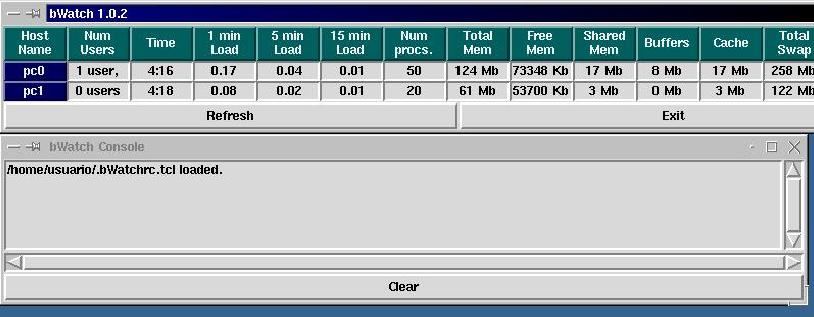
\epsfig{file=imagenes/bWatch/bWatch.eps, width=4.25in}
\caption{Monitorizaci�n Cluster}
\end{center}
\end{figure}
\clearpage